\documentclass{report}
\usepackage[utf8]{inputenc}
\usepackage{graphicx}

\graphicspath{ {image/} }

\title{First Document}
\author{Matt Chan \thanks{Overleaf Tutorial}}
\date{August 2019}

\begin{document}

\maketitle

\begin{abstract}
This is a simple paragraph at the beginning of the document. A brief introduction about the main subject.    
\end{abstract}

First document. This is a simple example, with no extra parameters or packages included.

Some of the \textbf{greatest} discoveries in \underline{science} were made by \textbf{\textit{accident}}.
Some of the greatest \emph{discoveries} in science were made by accident.
\textit{Some of the greatest \emph{discoveries} in science were made by accident.}
\textbf{Some of the greatest \emph{discoveries} in science were made by accident.}

The universe is immense and it seems to be homogeneous, in a large scale, everywhere we look at.

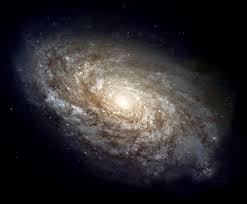
\includegraphics{image/galaxy.jpg}

There's a picture of a galaxy above.

\begin{figure}[h]
    \centering
    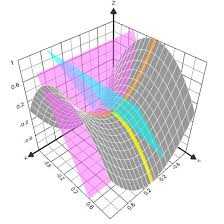
\includegraphics[width=0.25\textwidth]{image/graph.jpg}
    \caption{A nice plot.}
    \label{fig:plot1}
\end{figure}

As you can see in the figure \ref{fig:plot1}, the function grows near 0. Also, in the page \pageref{fig:plot1} is the same example.

\begin{itemize}
    \item The individual entries are indicated with a black dot, a so-called bullet.
    \item The text in the entries may be of any length.
\end{itemize}

\begin{enumerate}
    \item This is the first entry in our list
    \item The list numbers increase with each entry we add
\end{enumerate}

In physics, the mass-energy equivalence is stated by the equation $E=mc^2$, discovered in 1905 by Albert Einstein.

The mass-energy equivalence is described by the famous equation

\[E=mc^2\]

discovered in 1905 by Albert Einstein.
In natural units ($c = 1$), the formula expresses the identity

\begin{equation}
    E=m
\end{equation}

Subscripts in math mode are written as $a_b$ and superscripts are written as $a^b$. These can be combined and nested to write expressions such as

\begin{equation}
    T^{i_1 i_2 \dots i_p}_{j_1 j_2 \dots j_q} =
    T(x^{i_1}, \dots, x^{i_p}, e_{j_1}, \dots, e_{j_q})
\end{equation}

We write integrals using $\int$ and fractions using $\frac{a}{b}$. Limits are placed on integrals using superscripts and subscripts:

\begin{equation}
    \int_0^1 \frac{1}{e^x} = \frac{e-1}{e}
\end{equation}

Lower case Greek letters are written as $\omega$ $\delta$ etc. while upper case Greek letters are written as $\Omega$ $\Delta$.

Mathematical operators are prefixed with a backlash as $\sin(\beta)$, $\cos(\alpha)$, $\log(x)$ etc.

\tableofcontents

\chapter{First Chapter}

\section{Introduction}

This is the first section.

Lorem ipsum dolor sit amet, consectetur adipisicing elit, sed do eiusmod tempor incididunt ut labore et dolore magna aliqua. Ut enim ad minim veniam, quis nostrud exercitation ullamco laboris nisi ut aliquip ex ea commodo consequat. Duis aute irure dolor in reprehenderit in voluptate velit esse cillum dolore eu fugiat nulla pariatur. Excepteur sint occaecat cupidatat non proident, sunt in culpa qui officia deserunt mollit anim id est laborum.

\section{Second Section}
Lorem ipsum dolor sit amet, consectetur adipisicing elit, sed do eiusmod
tempor incididunt ut labore et dolore magna aliqua. Ut enim ad minim veniam,
quis nostrud exercitation ullamco laboris nisi ut aliquip ex ea commodo
consequat. Duis aute irure dolor in reprehenderit in voluptate velit esse
cillum dolore eu fugiat nulla pariatur. Excepteur sint occaecat cupidatat non
proident, sunt in culpa qui officia deserunt mollit anim id est laborum.

\subsection{First Subsection}
Lorem ipsum dolor sit amet, consectetur adipisicing elit, sed do eiusmod
tempor incididunt ut labore et dolore magna aliqua. Ut enim ad minim veniam,
quis nostrud exercitation ullamco laboris nisi ut aliquip ex ea commodo
consequat. Duis aute irure dolor in reprehenderit in voluptate velit esse
cillum dolore eu fugiat nulla pariatur. Excepteur sint occaecat cupidatat non
proident, sunt in culpa qui officia deserunt mollit anim id est laborum.

\addcontentsline{toc}{section}{Unnumbered Section}
\section*{Unnumbered Section}
Lorem ipsum dolor sit amet, consectetur adipisicing elit, sed do eiusmod
tempor incididunt ut labore et dolore magna aliqua. Ut enim ad minim veniam,
quis nostrud exercitation ullamco laboris nisi ut aliquip ex ea commodo
consequat. Duis aute irure dolor in reprehenderit in voluptate velit esse
cillum dolore eu fugiat nulla pariatur. Excepteur sint occaecat cupidatat non
proident, sunt in culpa qui officia deserunt mollit anim id est laborum.

\begin{center}
    \begin{tabular}{ c c c }
        cell1 & cell2 & cell3 \\
        cell4 & cell5 & cell6 \\
        cell7 & cell8 & cell9    
    \end{tabular}    
\end{center}

\begin{center}
    \begin{tabular}{ |c|c|c| }
        \hline
        cell1 & cell2 & cell3 \\
        cell4 & cell5 & cell6 \\
        cell7 & cell8 & cell9 \\
        \hline    
    \end{tabular}    
\end{center}

Table \ref{table:data} is an example of referenced \LaTeX{} elements.

\begin{table}[h!]
    \centering
    \begin{tabular}{||c c c c||}
        \hline
        Col1 & Col2 & Col3 & Col4 \\ [0.5ex]
        \hline\hline
        1 & 6 & 87837 & 787 \\
        \hline
        2 & 7 & 78 & 5415 \\
        \hline
        3 & 545 & 778 & 7507 \\
        \hline
        4 & 545 & 18744 & 7560 \\
        \hline
        5 & 88 & 788 & 6344 \\ [1ex]
        \hline        
    \end{tabular}
    \caption{Table to test captions and labels}
    \label{table:data}    
\end{table}



\end{document}